\documentclass[12pt, titlepage]{article}
\usepackage[french]{babel}
\usepackage[utf8]{inputenc}
\usepackage{fullpage}
\usepackage{setspace}
\usepackage{graphicx}
\usepackage{subfigure}
\usepackage{setspace}
\usepackage{tabularx}
\usepackage{hyperref}
\usepackage{times}
\usepackage{textcomp}
\usepackage{float}
\usepackage{capt-of}
\usepackage[toc,page]{appendix} 
\usepackage{lipsum}
\usepackage{booktabs}
\usepackage{enumitem}
\setlength{\parskip}{0.2cm}
\linespread{1.3}


% Taken from	tex.stackexchange.com/questions/88414/how-can-i-create-a-question-answer-format-for-reports
\newenvironment{QandA}{\begin{enumerate}[label=\bfseries\alph*.]\bfseries}
                      {\end{enumerate}}
\newenvironment{answered}{\par\normalfont}{}
\graphicspath{ {../captures/} }
% % % % % % % Début des commandes % % % % % %
	\newcommand{\Poly}{École Polytechnique de Montréal}
	\newcommand{\SigleCours}{INF8500}
	\newcommand{\NomCours}{Systèmes embarqués: Conception et vérification}
	

        \newcommand{\uwriter}{Uart\_Write }
        \newcommand{\udriver}{Uart\_Driver }
        \newcommand{\ucheck}{Uart\_Check }
        \newcommand{\theDut}{Uart }
        \newcommand{\uconfig}{Uart\_config }
        \newcommand{\refToStep}[2]{\hyperref[#1]{Étape \ref{#1}: #2}}
        \newcommand{\mss}{millisecondes }
        \newcommand{\cvp}{\emph{coverpoint }}                \newcommand{\cvg}{\emph{covergroup }}	
% % % % % % % Fin des commandes % % % % % %

\title{\Poly \\ \SigleCours --- \NomCours\\ \emph{TP1} }
\author{
\begin{tabular}
{l r}
Emilio Rivera & 1689355 \\ 
Théophile Gindre & 1864282 \\
Clément Gamache & 1642792 \\
\end{tabular}
\\ \\ \\ \\}
	\hypersetup{
		colorlinks,
		citecolor=black,
		filecolor=black,
		linkcolor=black,
		urlcolor=black
	}

\begin{document}
	\maketitle
        \begin{singlespacing}
	  \tableofcontents
        \end{singlespacing}
        \newpage
        \section{Analyse du DUT}
    	% Estimation des paramètres
	%\begin{figure}[H]
	%  \centering
	%  \includegraphics[width = \textwidth]{estimationParametre.png}
	%  \caption{Estimation des paramètres $\mu$ et $\sigma$ du taux d'homicide}
	%  \label{Estimation Parametre}
	%\end{figure}
	% Fin de l'estimation des paramètres
        
        Afin de démontrer le comportement de \emph{loopback} entre les broches d'envoi et de réception du UART, divisons le processus en plusieurs parties :
        \begin{enumerate}
          \item \label{rxtx:firststep} \udriver : Envoi du nombre par bus vers \theDut
          \item \label{rxtx:secondstep} \theDut : Réception et écriture en série vers \udriver
          \item \label{rxtx:thirdstep}\udriver : Réception du nombre
        \end{enumerate}
        L'étape \ref{rxtx:firststep} est possible d'être vue...
        L'étape \ref{rxtx:secondstep} est possible d'être vue...
        L'étape \ref{rxtx:thirdstep} est possible d'être vue...

        
        Comme il est possible de le voir à la \hyperref[rxtx:rxtxscreenshot]{figure \ref{rxtx:rxtxscreenshot}}, le signal de RX est égal en tout temps au signal TX
        
	    \begin{figure}[h]
	    	\centering
		    \caption{Mise en évidence de la relation entre le fil RX et TX}
	    	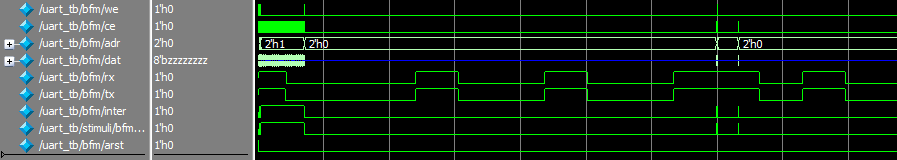
\includegraphics[ width= \textwidth]{rxIsTx.png}
    		\label{rxtx:rxtxscreenshot}
	    \end{figure}

		 \begin{figure}[h]
			\centering
			\caption{\refToStep{rxtx:firststep}{Écriture de la valeur 9 par \udriver vers \theDut}}
			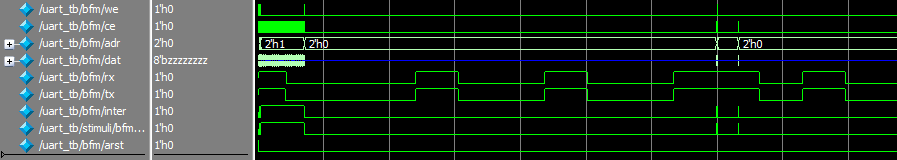
\includegraphics[ width= \textwidth]{rxIsTx.png}
			\label{rxtx:firststepscreenshot}
		\end{figure}
	
		\begin{figure}[h]
			\centering
			\caption{\refToStep{rxtx:secondstep}{Transmission sérielle par \theDut vers \udriver}}
			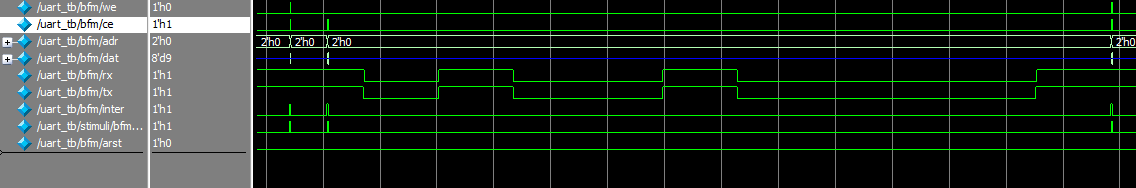
\includegraphics[ width= \textwidth]{serial9.png}
			\label{rxtx:secondscreenshot}
		\end{figure}
	
		\begin{figure}[h]
			\centering
			\caption{\refToStep{rxtx:thirdstep}{Lecture par \udriver de la valeur transmise sériellement}}
			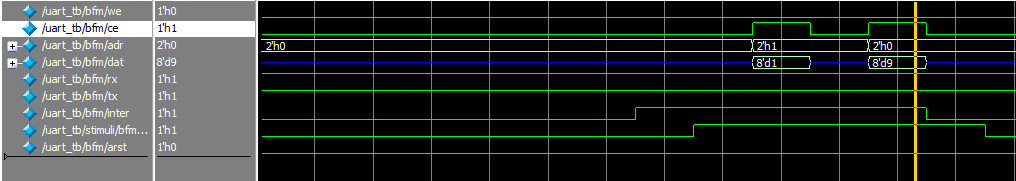
\includegraphics[ width= \textwidth]{read9.png}
			\label{rxtx:thirdstepscreenshot}
		\end{figure}

\section{Modification du DUT pour plan de test}
    \subsection{Test de transmission}
        \lipsum[1] 
    \subsection{Test de réception}
    % TODO
        Plusieurs problèmes ont été recontrés:
        \begin{itemize}
        \item Création et transfert de l'interface
        \item Synchronisation entre les UART et les mailbox (utilisation de sémaphore) + une nouvelle mailbox entre \udriver et \ucheck.
        \item Connexion entre les deux UART
        \end{itemize}

\section{Amélioration de la génération aléatoire} 
    \subsection{Création de la classe \uconfig} 
    La création de la classe \uconfig a été facile. La création de l'objet dans le programme de test est possible à partir de la méthode new(). Cette dernière mets des valeurs par défaut dans les membres de classe (qui sont décrits dans la prochaine section).

    Une subtilité à prendre en compte, qui est cependant expliquée dans la documentation, est la façon dont il faut déclarer les membres de la classe. En effet, afin que l'appel à randomize() change la valeur des attributs, il faut que ces derniers soient définis comme rand ; le type des attributs doit être précédé par "rand".
    
    \subsection{Contenu de la classe \uconfig}
    Des membres de type enum ont été ajoutés dans la classe de configuration. Un comportement intéressant de la fonction randomize() appliquée sur des enums est le fait qu'une valeur aléatoire est choisie parmi les valeurs possibles de la structure. Ainsi, randomize() appliquée sur un enum avec quatre possibilités retourne toujours une de ces quatre possibilités.
    \subsection{Modification de l'initialisation des modules} 
    Puisque les configurations affectent la vitesse de transmission, il fallait que \udriver puisse avoir accès à cette nouvelle information. Dans la fonction d'initialisation de \udriver, une classe qui contient la configuration est passée en paramètre. C'est \udriver qui est en charge d'écrire sa configuration dans la mémoire. Un simple décalage binaire de trois (afin d'écrire dans le troisième bit[il s'agit du bit de configuration de la parité]) suffit.

    
    \subsection{Modification du programme de test}
    Dans le code initial, une seule exécution des modules étaient faite. C'est-à-dire que le testbench finissait quand l'un des modules avait terminer. Afin de faire plusieurs types de configuration, nous avons choisi d'englober le tout dans un block repeat. Bien entendu, les configurations étaient changées à chaque itération à l'aide de randomize().

    La création des modules a été bougée avant le bloc repeat, car il s'agissait de destruction et création de modules inutiles. En effet, il suffit dans notre cas que d'appeler la nouvellement modifiée méthode d'initialisation afin de changer la configuration des modules.
    
    Après avoir fait cette modification, un autre problème survint : les temps d'éxecution de chaque boucle était considérablement long. En effet, dans le code précédent, \uwriter attendait 200 ms avant de terminer. Nous avons donc réduit cette valeur à 20 ms. 

    Par la suite, des problèmes de synchronisation furent détectées. Après avoir analysé les sorties sur la console des différentes valeurs testées dans les mailboxs, il nous apparut que lorsqu'une boucle du repeat était terminée, les mailbox n'étaient pas vidées. Par exemple, pour la deuxième configuration testée, la première valeur lue par \ucheck correspondait à l'avant dernière donnée envoyée par \udriver dans l'itération précédente. À premier regard, le fait de vider les mailbox serait suffisant, mais cela ne permettrait pas à \ucheck de recevoir les dernières données envoyées. Il fut donc déterminé qu'il fallait attendre que \ucheck ait reçu toutes les données envoyées (c'est d'ailleurs la raison de l'existence de l'attente de 200 ms dans le code original). Un fork avec une attente complète (join / join-all )a donc été imbriqué dans le programme de test sur \uwriter et \ucheck (\udriver et le receiver roulent à l'infini). 


    \subsection{Vérification du changement de parité} 
		\begin{figure}[h]
			\centering
			\caption{Mise en évidence de la parité}
			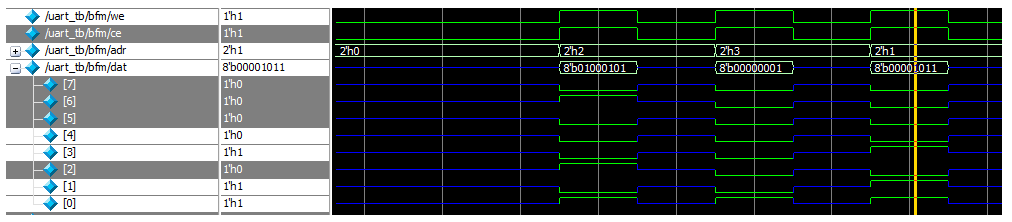
\includegraphics[ width= \textwidth]{parity.png}
			\label{random:parity}
		\end{figure}
        Comme il est possible de voir à la \hyperref[random:parity]{figure \ref{random:parity}}, le bit de parité (index 3) est mis à 1, ce qui indique une activation de la parité.
    \subsection{Méchanisme de génération aléatoire}
    En effet, il a été remarqué qu'à travers les multiples simulations, les mêmes valeurs apparaissaient. Il s'agit d'un mécanisme très intéressant dans le cadre de la vérification car les mêmes ensembles de données sont utilisées : si un problème est détecté dans l'un de ensembles, il est possible de relancer la simulation et d'obtenir exactement le même problème pour le même ensemble. Si les données étaient réellement aléatoires, obtenir de nouveau le problème serait une question de chance. Ceci facilite énormément le travail des personnes qui font la vérification, car reproduire le problème est parfois un long trajet.

    Il est possible de le faire en changeant la graine du simulateur (qui détermine la graine des modules) :

    \texttt{sim switch -sv\_seed [value]}
    
    Même si le testbench change, les valeurs aléatoires restent les même. En effet, ce n'est pas la compilation qui change la génération de nombre : il s'agit de la graine de génération. Cette graine est spécifique à la simulation. Comme précédemment expliqué, il s'agit d'une trés bonne fonctionnalité car elle assure la reproductibilité de la simulation. Il est par ailleurs possible de changer cette grain entre les simulations.
    
    % http://www.doulos.com/knowhow/sysverilog/SNUG13_random_stability/SNUG2013_SV_Random_Stability_paper.pdf

\section{Injection d'erreurs} 
	
	
	
	La plus grande difficulté fût la synchronisation entre les bits pour l'injection. Il ne s'agit pas de la première synchronisation, car cette dernière est facile à détecter : il suffit d'attendre un changement de valeur pour la transmission sur le fil de transmission du UART de référence avec \emph{negedge}.
	
	 Afin que le module d'injection modifie correctement au bon moment, notre diviseur devait être aligné avec le baudrate de transmission. Le premier réflèxe fût d'essayer de calculer exactement le temps nécessaire, mais lors des tentatives d'injection, les mauvais bits étaient changés. 
	
	Il a ensuite été décidé de vérifier la validité de notre valeur en regardant la \emph{waveform}. Suite à l'observation de cette dernière, nous avons vu que la valeur calculée théoriquement était peu éloignée (à $ \pm5 \%$). Des tentatives de calcul furent éffectuées afin de découvrir comment la valeur exacte devait être obtenue, mais en vain. Les valeurs finales furent donc extraites manuellement depuis les \emph{waveform}.
    \subsection{Injection du Parity Error} 
    	Il s'agit de le bit indiquant la parité du message : chaque transmission complète est constituée de 11 bits dans lesquels 8 constituent le message, 2 démarquent le début et la fin et 1 indique la parité du message. 
    	Ainsi, en changeant le bit de parité (le neuvième à passer dans le fil dans chaque transmission), \theDut devrait être en mesure de détecter l'erreur.
    	    	
    \subsection{Injection du Framing Error} 
    	Il s'agit simplement de faire un décalage dans la transmission vers \theDut : cela est possible en utilisant l'instruction \emph{wait} lors de la transmission d'un bit. 

    \subsection{Injection du Data Error} 
    	Il s'agit simplement d'inverser un bit dans le message envoyé à \theDut et de vérifier si ce dernier le détecte. Puisqu'il s'agit d'une vérification par parité, un nombre impair de bits doit être changé. Il fût décidé qu'un seul bit serait changé.

\section{Couverture}
    \subsection{Groupe de couverture} 
    	Un \cvg a été créé dans la classe de configuration. Nous avons laissé Questa généré les \emph{bins} automatiquement, cela pour le \emph{baudrate} et pour la configuration d'erreurs. Pour le \emph{baudrate}, Questa génère un \emph{bin} par valeur de baudrate. Par la suite, un produit cartésion a été utilisé comme troisième \cvp ce qui résulte en $4 * 5 = 20$ possibilités. 
		Le programme de test a été modifié afin d'avoir une couverture complète du nouveau \cvg : la configuration est générée aléatoirement, un test est fait et échantillonné, le tout tant que la couverture est inférieure à 100\%.
		
		Dans un cas idéal, nous aurions besoin de 20 itérations afin de tester entièrement le \cvg en question. Dans notre cas, 59 itérations furent nécessaires avant d'obtenir une couverture complète.
		
		Étant donné notre architecture du banc de test, nos \cvp entre le \emph{receiver} et le \emph{driver} étaient différents. Ceci est dû au fait que \udriver faisait une attente bloquante sur une \emph{mailbox} et par la suite effectuait un échantillonage. Tandis que \emph{receiver} s'agissait d'une tâche qui roulait en permanence sans blocage : le nombre d'échantillons prélevés est considérablement supérieur au nombre d'échantillons de \udriver. 

		% TODO
		
		Il fut remarquer que la couverture du \cvp de \udriver était minimal : cela était du au fait que \udriver était en attente d'un message de \uwriter lorsque des erreurs étaient présentes ; il n'échantillonait pas lorsque des erreurs étaient injectées. Il fut donc décider de faire l'échantillonage uniquement sur le \emph{receiver} puisqu'il roule tout le temps. 

		La relation n'est pas parfaite : une erreur de parité peut être causée par les trois types d'erreurs injectées.
		Évidemment, une erreur sur le bit indiquant la parité du message indiquera une erreur sur la parité (si le bit de parité est lu).
		Une \emph{DATA ERROR} cause aussi une erreur sur la parité puisque notre façon d'injecter une erreur était de modifier un bit : inverser un nombre impair de bits causera une erreur sur la parité.
		Finalemenent, une injection d'erreur sur le \emph{framing} pourrait causer une erreur sur la parité : un bit serait sauté dans le message et causerait possiblement une erreur sur le message, ce qui pourrait influencer la parité du message.
		
    \subsection{Automatisation de la fin de test} 
    	Il est simplement possible d'utiliser la fonction \emph{get\_inst\_cov} afin d'obtenir la couverture jusqu'à présent et d'utiliser un compteur d'itération afin de délimiter la boucle du programme de test.
    	
    	 \begin{table}[h!]
			 	\begin{center}
			 		\caption{Positions des pouvant être ionisés sur leur chaîne latérale}
			 		\label{tab:posIonisables}
			 		\begin{tabular}{c|c}
			 			Couverture (\%) & Itérations nécessaires\\
			 			\midrule
						   100   & 59 \\
			 		\end{tabular}
			 	\end{center}
		 \end{table}
    	
\section{Assertions}
    TODO
\end{document} 
